\chapter{RESULTADOS E Discussões}\label{ch:intro}
Utilizando os materiais e métodos previamente apresentados, neste capítulo serão
apresentados e discutidos os resultados obtidos a partir dos experimentos abordados na base de imagens criada, assim como comparações com os efeitos de processamento de imagens aplicados na base de imagens coletada. Os resultados serão apresentados na ordem de imagens classificadas em ambiente de luminosidade favoráveis até as imagens capturadas em ambiente noturno.


As métricas apresentadas foram calculadas obtendo-se uma média de acertividade do resgate correto dos caracteres do nome do medicamento em questão, analisando a quantidade de caracteres e quantidade de resgates corretos.

 No decorrer da criação da base de imagens, foi constatado que o dispositivo celular Samsung J2  não possui boa captura de imagens em ambientes com baixa luminosidade, mas ainda assim optou-se por continuar com a captura de imagens e os testes, pelo fato de poder reproduzir uma situação real, que pode ocorrer com futuros usuários da aplicação em estudo.
 
Os testes foram realizados e comparados entre as categorias de imagens, perspectivas e entre as técnicas de processamento de imagem. Os testes foram encerrados quando três testes consecutivos da mesma categoria de imagens não obtiveram resgates de pelo menos 3 caracteres corretos e sequentes, o que impossibilitou o próximo passo, que é a recuperaração dos registros na base de dados descritiva dos medicamentos.

%EVERTON: O usuário precisará ter no dispositivo dele a base de todas as imagens?
Em todos os experimentos que serão apresentados, foi necessário importar as fotos do banco de imagens para o projeto como forma de asset, que é a forma correta onde um aplicativo de celular identifica e caracteriza uma imagem internamente para importação. Como forma de simplificar posteriormente as buscas na base de informações de remédios, foram ignorados os acentos, o que não impactará nos resultados do OCR demonstrados a seguir. Dessa maneira, caso o OCR identifique alguma letra que possua acento, é realizado um pós processamento no texto para que a consulta seja feita sem acentos e caracteres especiais, visando deixar a busca simplificada e com um poder acertivo maior.

\section{MANIPULAÇÃO DOS DADOS COLETADOS}

Segundo o Portal da \citeonline{PORTALANVISA}, desde o ano 2000 até 05/08/2019, 5.723 medicamentos genéricos foram registrados. Destes, 2.398 registros foram cancelados, restando 3.325 medicamentos genéricos com registros válidos. Em base dessa informação, pensando em trabalhos futuros e pensando em ganho de desempenho no dispositivo celular, foi optado por manipular os dados via \textit{JSON}, viabilizando de forma mais dinâmica o uso de banco de dados não relacionais, chamados de NoSQL, que trabalham diretamente com arquivos JSON.

Os dados coletados para este trabalho foram capturados manualmente do bulário da Anvisa e % -> escritos no salvos <- % no tipo JSON para facilitar a busca detalhada pela lista de objetos criadas do tipo Medicamento, onde possui as seguintes chaves de identificação:

\begin{lstlisting}[firstnumber=1]
{
  "medicamentos": [
      {"id": 1},
      {"nome": "descricao"},
      {"principios_ativos": "descricao"},
      {"contra_indicacoes": "descricao"},
      {"tipo_medicamento": "descricao"},
      {"data": "descricao"}
    ]
}
\end{lstlisting}
\fonte{Autoria Própia.}


Com retorno obtido do OCR Firebase MLKit, é possível obter os textos em blocos, linhas e palavras, conforme descrito na sessão 2.5.2, possibilitando realizar uma rápida busca no documento \textit{JSON} local. Por este motivo, foi elaborado um processo com 6 algoritmos de pós processamento dos dados, no intuito de efetuar uma busca mais refinada e acertiva dos dados coletados do OCR na base de dados JSON, que são:

\begin{enumerate}
  \item Limpeza dos dados coletados;
  \item Busca simples por palavras;
  \item Substituição de números visualmente similares a letras;
  \item Busca por palavras formatadas;
  \item Busca contendo a metade das letras iniciais das palavras;
  \item Busca contendo a metade das letras finais de cada palavra.
\end{enumerate}

%EVERTON: Você usa muito feito. Feito é fazer, construir. Procure melhorar esta situação no documento.
Na primeira etapa, algumas palavras padrões foram identificadas durante o estudo das caixas de medicamento como por exemplo: "VENDA SOB PRESCRIÇÃO MÉDICA", "50 mg", "Uso Oral", "Uso adulto" e "Contém 20 comprimidos". Essas palavras serão excluídas neste trabalho, porém elas podem servir de informações adicionais e podem ser relevantes para um sistema mais criterioso em trabalhos futuros.

Supondo que uma caixa de medicamento não contenha mais de 50 palavras, na segunda etapa do processo foi analisado que se faz viável a comparação de todas as palavras encontradas com todos os registros de chave de valor "nome" do documento JSON. Mesmo que seja encontrado algum registro, será efetuado a terceira etapa.

Na terceira etapa, é feito um segundo refinamento das informações nas palavras encontradas, se possuir caracteres iguals ao número 0, substituir pela letra "O", número 1 pela letra "L", número 4 pela letra "A" e também o número 7 pela letra "T", devido ao seu alto grau de semelhança visual para o OCR. 

Após feito a troca dos caracteres, será feita uma nova busca na base de dados JSON, passando palavra por palavra que representa a quarta tarefa da lista. Caso não seja encontrado nenhum registro, o algoritmo % COMO ASSIM?? interpretará o quinto passo, que é a separação da palavra ao meio, formando 2 partes, do início da palavra até a metade e da metade até o final. Fazendo então ser possível a busca novamente na base por medicamentos que contenham essa sequência de letras na chave "nome" do documento JSON.

A cada Medicamento encontrado nas etapas, o medicamento é inserido em uma lista que por fim será apresentada para o usuário, retornando apenas os medicamentos distintos encontrados. Caso haja mais de um medicamento encontrado na base, será apresentado uma lista simples, para que o usuário selecione o medicamento correto.


\section{Experimento sem manipulação de imagem}
Os resultados apressentados na Tabela \ref{tab:exp_sem_filtro}, são referentes às imagens originais submetidas ao OCR, sem nenhum tipo de tratamento de imagem. A coluna sem processamento dos dados, está representada por "SP" e a coluna com o pós processamento de dados, está representada por "CP".


\begin{table}[]
\caption{Experimento sem aplicar filtro nas fotos}
\label{tab:exp_sem_filtro}
\centering
\begin{tabular}{llccc}
\hline
Categoria          & Tamanho    & Tempo (sec) & SP \%  & CP \% \\ \hline
Boa luminosidade   & 76,8 MB & 72     & 100 & 100         \\
Baixa luminosidade & 104 MB & 91     & 83,33 & 100         \\
Ambiente externo   & 88,9 MB & 80     & 100 & 100         \\
Noturnas sem flash & 82,9 MB & 78     & 83,33& 100         \\
Noturnas com flash & 96,7 MB & 87     & 83,33 & 100         \\ \hline
\end{tabular}
\fonte{Autoria Própria.}	
	\label{fig:exp_sem_filtro}
\end{table}

Foi identificado 


\section{EXPERIMENTO APLICANDO efeito DE ESCALAS EM CINZA}
%EVERTON: Não é primeira pessoa
Para aplicar o filtro de imagem em escalas de cinza, foi necessário implementar um algoritmo para tal função. Como estamos manipulando um objeto do tipo \textit{File} (arquivo) da galeria, foi necessário decodificar o \textit{File} e transformar para um objeto do tipo textit{Image}. 

Para otimizar tempo e recurso de memória do celular que acabou sendo insuficiente, foi necessário fazer uma transformada no tamanho da imagem, para altura igual a 600 e largura igual a 600. Com o array de bits gerado da imagem, foi possível iniciar a conversão da imagem para escala de cinza, conforme figura \ref{fig:greyscale}, deixando assim, a imagem em escala de cinza pronta para ser aplicada ao OCR.


% Deixo essa imagem? Não consegui transformar para pseudo código


 \begin{figure}[h]
	\centering
	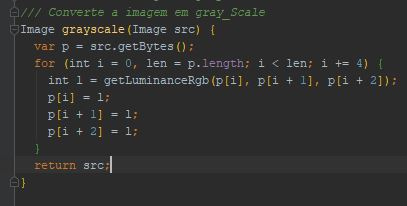
\includegraphics[width=0.6\textwidth]{Imagens/greyscale.JPG} % <- formatos PNG, JPG e PDF
	\caption[Algorítmo de conversão em escalas de cinza.]{Algorítmo de conversão em escalas de cinza.}
\fonte{Autoria Própria.}%citaç\~ao do livro onde pegou a figura	
	\label{fig:greyscale}
\end{figure}

Os resultados do experimento de pré processamento aplicando efeito de escalas em cinza na imagem, são apressentados na Tabela \ref{tab:exp_sem_filtro}.

\begin{table}[]
\caption{Experimento aplicando filtro de escalas em cinza.}
\label{tab:exp_grey_scale}
\centering
\begin{tabular}{llccc}
\hline
Categoria          & Tamanho    & Tempo (sec) & SP  & CP \% \\ \hline
Boa luminosidade   & 76,8 MB & 164     & 77 & 100         \\
Baixa luminosidade & 104 MB & 211     & 45 & 83,3         \\
Ambiente externo   & 88,9 MB & 181     & 77 & 100         \\
Noturnas sem flash & 82,9 MB & 600+     & 0& 0         \\
Noturnas com flash & 96,7 MB & 474     & 16,6 & 16,6         \\ \hline
\end{tabular}
\fonte{(Autoria Própria)}	
	\label{fig:exp_grey_scale}
\end{table}



\section{EXPERIMENTO APLICANDO efeito DE Sobel}

Para aplicar o efeito de Sobel na imagem, como proposto na sessão de materiais e métodos, foi necessário implementar um algoritmo para tal função. Também neste caso, como estamos manipulando um objeto do tipo \textit{File} da galeria, foi necessário decodificar o \textit{File} e transformar para um objeto do tipo \textit{Image}. Para otimizar tempo e recurso de memória, foi necessário fazer uma transformada no tamanho da imagem, para altura igual a 600 e largura igual a 600. Com o array de bits gerado da imagem, foi possível iniciar a conversão da imagem aplicando o filtro de Sobel. Deixando assim, a imagem com filtro de Sobel pronta para ser manipilada pelo OCR. 

\begin{table}[]
\caption{Experimento aplicando filtro de Sobel.}
\label{tab:exp_sobel}
\centering
\begin{tabular}{llccc}
\hline
Categoria          & Tamanho    & Tempo (sec) & SP\%  & CP \% \\ \hline
Boa luminosidade   & 76,8 MB & 451     & 0 & 0         \\
Baixa luminosidade & 104 MB & 570     & 0 & 0         \\
Ambiente externo   & 88,9 MB & 514     & 0 & 0         \\
Noturnas sem flash & 82,9 MB & 600+     & 0& 0         \\
Noturnas com flash & 96,7 MB & 600+     & 0 & 0         \\ \hline
\end{tabular}
\fonte{(Autoria Própria)}	
\end{table}

Como demonstrado na Tabela \ref{tab:exp_sobel}, houve uma grande complicação para processamento da imagem, tanto para a conversão quanto para o OCR de efetuar a extrassão dos caracteres nas imagens.

\chapter{CONSIDERAÇÕES FINAIS}\label{ch:intro}
Neste capítulo são resumidas as principais consideracões finais acerca do trabalho, bem como suas contribuicões sociais. Também é abordado possíveis trabalhos futuros para melhorar e dar continuidade ao objetivo de utilizar tecnicas de processamento de imagem juntamente com OCR no auxílio de uma classe social de idosos que vem crescendo continuamente no Brasil.


\section{CONCLUSÃO}

Este trabalho mostrou que é possível desenvolver técnicas de reconhecimento de caracteres em um ambiente offline acopladas a aplicativos, sendo possível auxiliar a população no processo medicamentoso. Com uma foto de boa qualidade, luminosidade e resolução maior que 5mp, é possível extrair o nome e informações adicionais da embalagem do medicamento em questão em pouco menos de 3 segundos, dando um amplo acesso a possibilidades para se trabalhar com esse tipo de dado e solucionando problemas sociais e empresariais.

Com o estudo implementado neste trabalho, é possível levar informação a uma grande parcela da população brasileira que por vezes não dispõe de capacidades visuais para ler letras miúdas de uma bula, pessoas não analfabetizadas, pessoas sem acesso a internet e até mesmo um aplicativo de auto ajuda para o dia a dia de agentes da saúde, que muitas vezes se encontram em locais remotos sem acesso a informações.  

Para o celular, além de complexo a nível de hardware limitado, efetuar técnicas de processamento de imagens se mostrou causar uma demora significativa para a tarefa e sendo menos eficiente do que imagens sem técnicas de processamento.

No conjunto de imagens expostas à técnicas de processamento de imagem, as imagens com pré processamento obtiveram menores taxas de acertividade e um tempo maior de processamento, uma vez que os recursos de processamento do aparelho celular são limitados para tal função. Por estes motivos, foi possível observar que o OCR da Google se saiu melhor em fotos de uso real do dia a dia.

Os testes realizados foram efetuados com caixas de medicamentos aleatórios, diferentes tamanhos, perspectivas, cores e tonalidades de contraste, o que não foi um grande desafio para o tema proposto.

Visando trabalhos futuros com consultas de bases de dados mais complexas e externas do celular, foi implementado a regra de estrutura de dados manipulando JSON, onde os dados serão muito melhor trafegados pela rede. Outro lado positivo estudado neste trabalho, foi o OCR do Firebase MLKIT, que apresentou um resultado excelente no resgate de caracteres, chegando quase a perfeição do reconhecimento dos caracteres a nível de nome do medicamento.

\section{trabalhos futuros}


Para possíveis trabalhos futuros baseados neste, se indica:

\begin{enumerate}
  \item Aplicar outros SDK de OCR para possíveis melhores resultados.
  \item Melhorar o algoritmo de busca em lista para ter uma melhor eficácia na identificação do medicamento, caso o OCR venha errar sequência de 3 letras ou mais da palavra do medicamento em questão.
  \item Generalizar o tema proposto, sendo possível trabalhar com diferentes categorias de imagens e com diferentes problemas sociais.
  \item Criar uma base de dados externa para consultas complexas que possa retornar mais informações do medicamento em questão ou até mesmo apresentar informações mais pertinentes, assim como cadastro de medicamentos não regulamentados pela Anvisa na base de dados descritiva dos medicamentos.
\end{enumerate}


